\documentclass{beamer}
%\usecolortheme{spruce}
\usetheme{A}

\usepackage{amsmath}
\usepackage{datetime}
\usepackage{relsize}
\usepackage{ulem}
\usepackage{amsmath}
\usepackage{calc}
\usepackage{tikz}
\usepackage{tabularx}
\usepackage{stmaryrd}
\usepackage{wasysym}
\usepackage{booktabs}
\usepackage{multicol}
\usepackage{colortbl}
\usepackage{proof}
\usepackage{relsize}
\usepackage{pgfplots}

\usepackage{fontspec}
\newfontfamily\DejaSans{DejaVu Sans}
\usetikzlibrary{calc}
\usepackage{pifont}% http://ctan.org/pkg/pifont

\definecolor{darkgreen}{HTML}{009900}
\definecolor{darkred}{HTML}{e60000}
\definecolor{darkyellow}{HTML}{ff9900}

\definecolor{rp}{HTML}{9400D3}
\definecolor{rp2}{HTML}{4B0082}
\definecolor{rb}{HTML}{0000FF}
\definecolor{rg}{HTML}{00FF00}
\definecolor{ry}{HTML}{FF7300}
\definecolor{ro}{HTML}{FF7F00}
\definecolor{rr}{HTML}{FF0000}

\newcommand{\dg}[1]{\textcolor{darkgreen}{#1}}
\newcommand{\dr}[1]{\textcolor{darkred}{#1}}
\newcommand{\dy}[1]{\textcolor{darkyellow}{#1}}
\newcommand{\happy}{\dg{\smiley}}
\newcommand{\sad}{\dr{\frownie}}
\newcommand{\term}[1]{\ensuremath{\mathtt{#1}}}
\newcommand{\li}{\multimap}
\newcommand{\lotimes}{\!\otimes\!}
\newcommand{\loplus}{\!\oplus\!}
\newcommand{\lin}[1]{\langle#1\rangle}
\newcommand{\lint}[1]{[#1]}
\newcommand{\cat}[1]{\footnotesize \textsc{#1}}	
\newcommand{\W}[1]{\scriptsize #1}
\newcommand{\etext}[1]{\scriptsize {\textit{#1}}}
\newcommand{\smain}{\cat{S}$_{\text{main}}$}
\newcommand{\ssub}{\cat{S}$_{\text{sub}}$}
\newcommand{\type}[2]{\scriptsize\ensuremath{\textcolor{#2}{#1}}}
\newcommand{\red}[1]{\textcolor{red}{{}_#1}}

%{\DejaSans ☺😐☹😁😂😃😇😉😈😋😍😱}

\newcommand{\cmark}{\ding{51}}%
\newcommand{\xmark}{\ding{55}}%

\newcolumntype{L}{>{\raggedright\arraybackslash}X}
\newcommand{\hnorm}{\vphantom{()}}
\newcommand{\dgat}[2]{\alt<#1>{\dg{#2}}{#2}}
\newcommand{\drat}[2]{\alt<#1>{\dr{#2}}{#2}}
\newcommand{\boxat}[2]{\ensuremath{\alt<#1>{\boxed{#2}}{#2}}}
\newcommand{\qmarkat}[2]{\alt<#1>{#2}{???}}
\newcommand{\gqmarkat}[2]{\dg{\alt<#1>{#2}{???}}}
\newcommand{\rqmarkat}[2]{\dr{\alt<#1>{#2}{???}}}

\hypersetup{
    colorlinks=true,
    urlcolor=blue,
    pdfpagemode=FullScreen,
}


\begin{document}



\date{\smaller End-to-End Compositional Models of Vector-Based Semantics\\
ESSLLI, August 2022, Galway}

\title{}
\subtitle{\textit{the \textcolor{rp}{u}\textcolor{rp2}{n}\textcolor{rb}{i}\textcolor{rg}{c}\textcolor{ry}{o}\textcolor{ro}{r}\textcolor{rr}{n} of constant-time parsing}}

\author{%
    Konstantinos Kogkalidis\\ 
    \inst{Utrecht Institute of Linguistics OTS, Utrecht University}
}


{%
\setbeamertemplate{headline}{}
\frame{\titlepage
\hspace{-10pt}
\begin{minipage}{0.5\textwidth}
\begin{minipage}{0.35\textwidth}

\includegraphics[scale=0.065]{NWO logo - RGB_wit_rondom_0.jpg}%
\end{minipage}%
\begin{minipage}{0.65\textwidth}
\smaller[3]
\centering
A composition calculus for vector-based semantic modelling
with a localization for Dutch\\
\end{minipage}
\end{minipage}%
\hfill
\begin{minipage}{0.45\textwidth}
\hfill
\raisebox{-5.5pt}{
\includegraphics[scale=0.5]{UU_logo_2021_EN_RGB.jpg}}
\end{minipage}%
}
}

\begin{frame}{Overview}
\begin{itemize}
\item Grammar
\item Supertagging
\item Parsing
\item Unicorns
\end{itemize}
\end{frame}

\section{Grammar}

\begin{frame}{A type grammar for the 21st century}
\smaller	

	ILL$_{\li}$ plus $\Diamond, \Box$ modalities for \textit{dependency domain demarcation}.
\vfill
	
Types inductively defined by:
\[
	\mathbb{T} := A \ | \  T \li T \ | \ \diamondsuit^d  T \ | \ \Box^d T \qquad A \in \mathbb{A}, T \in \mathbb{T}
\]
\vfill	

	\begin{itemize}
	\item[$\li$]		-- linear function builder
	\item[$\diamondsuit$] 	-- reserved for "necessary arguments", i.e. complements
	\item[$\Box$]		-- reserved for "optional functors", i.e. adjuncts
\end{itemize}
\end{frame}

\begin{frame}{..and its term calculus}
\smaller

\renewcommand{\arraystretch}{1.15}
{
\begin{tabularx}{\textwidth}{@{}c@{\qquad}c@{}}
$\infer[Lex]{\term{c}: T \vdash \term{c}: T}	{\vphantom{T}}$
&
\uncover<2->{
$\infer[\li E]{\Gamma, \Delta \vdash \term{s\ t}: T_2}{\Gamma \vdash \term{s}: T_1 \li T_2 & \Delta \vdash \term{t}: T_1}$}
\\
\\
\uncover<3->{
$\infer[\diamondsuit^d I]{\langle \Gamma \rangle^{d} \vdash \vartriangle^d \term{t}: \diamondsuit^d T}{\Gamma \vdash \term{t}: T}$
}
&
\uncover<4->{
$\infer[\Box^d E]{\langle \Gamma \rangle^d \vdash \blacktriangledown^d \term{s}: T}{\Gamma \vdash \term{s}: \Box^d T}$}
\\
\\
\uncover<5->{
$\infer[Ax]{\term{x}: T \vdash \term{x}: T}	{\vphantom{T}}$}
&
\uncover<6->{
$\infer[\li I]{\Gamma \vdash \lambda\term{x.s}: T_1 \li T_2}{\Gamma, \term{x}: T_1 \vdash \term{s}: T_2}$	}
\\
\\
\textcolor{gray!30}{
$\infer[\Box^d I]{\Gamma \vdash \blacktriangle^d \term{s}: \Box^d T}{\langle \Gamma \rangle^d \vdash \term{s}: T}$}
&
\textcolor{gray!30}{
$\infer[\diamondsuit^d E]{\Gamma[\Delta] \vdash \term{t}[\term{x} \mapsto \triangledown^d \term{s}]: T_2}{
		\Gamma[\langle \term{x}: T_1 \rangle^d] \vdash \term{t}: T_2			
		&\quad
		\Delta \vdash \term{s}: \diamondsuit^d T_1}$
}
\\
\\
\multicolumn{2}{c}{
\textcolor{gray!30}{
$\infer[\mathsf{X}]{\langle\Gamma, \Delta\rangle^d,  \langle \term{x}: T_1 \rangle^\mathsf{X} \vdash \term{s}: T_2}{
\langle\Gamma, \langle \term{x}: T_1 \rangle^\mathsf{X}, \Delta\rangle^d \vdash \term{s}: T_2}$}}
\end{tabularx}}
\end{frame}


\begin{frame}{Example}
	example too big, send help
\end{frame}


\begin{frame}{Now what?}

	The standard categorial pipeline:
\smaller
\begin{itemize}
	\item read a sentence
	\item \drat{2}{assign a type to each word}
	\item perform (a) phrasal composition
	\item ???
	\item profit
\end{itemize}

    \noindent
    \hfill\makebox[30pt][l]{%
      \raisebox{0pt}[60pt][0pt]{%
        \includegraphics[scale=0.2]{gnome.png}}
    }
    
\end{frame}

\section{Supertagging}


\begin{frame}{(pre-)history}
\smaller
    $
    p(t_1, \dots t_n ~ | ~ w_1, \dots w_n) \approx
    $
    
    \begin{itemize}
        \uncover<2->{
        \item $\prod_i^n (t_i~|~w_i)$\\
        \quad \textit{co-occurrence-based statistical models (90s)}}
        \uncover<3->{
        \item $\prod_i^n (t_i~|~w_{i-\kappa} \dots w_{i+\kappa})$\\
        \quad \textit{window-based n-gram models (00s), ffns (early 10s)}}
        \uncover<4->{
        \item $\prod_i^n (t_i~|~w_1,\dots w_n)$\\
        \quad \textit{sequence encoders (mid 10s)}}
        \uncover<6->{
        \item $\prod_i^n (t_i~|~t_1, \dots t_{i-1}, w_1,\dots w_n)$\\ 
        \quad \textit{seq2seq (late 10s)}}
    \end{itemize}
    \vfill

	\alt<11->{
what have we done?
\begin{itemize}
        \item[$\bullet$] more arrows (=more context)
        \item[$\bullet$] auto-regression (price: temporal delay)
        \item[$\bullet$] what about the co-domain?	
\end{itemize}
}
{
      \centering
        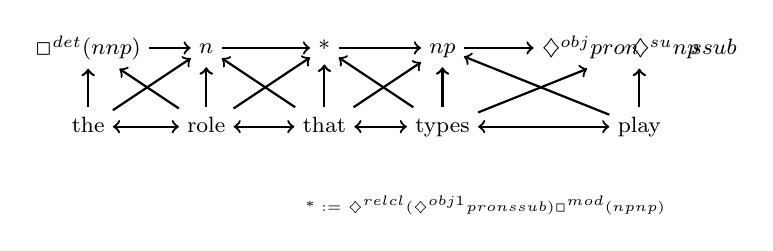
\begin{tikzpicture}
        [ctx/.style={thick, ->},
         ctxbi/.style={thick, <->}]
        	\smaller
        		\node			(w1)				at (-8.5, 0)  	{\hnorm the};
        		\node			(t1)				at (-8.5, 1)	{$\Box^{det} (n \li np)$};
        		\node			(w2)				at (-7,0)		{\hnorm role};
        		\node			(t2)				at (-7, 1)		{\hnorm $n$};
        		\node			(w3)				at (-5.5, 0)	{\hnorm that};
        		\node			(t3)				at (-5.5, 1)	{*};
        		\node			(w4)				at (-4, 0)		{\hnorm types};
        		\node			(t4)				at (-4, 1)		{\hnorm $np$};
        		\node			(w5)				at (-1.5, 0)	{\hnorm play};
        		\node			(t5)				at (-1.5, 1)	{\hnorm $\diamondsuit^{obj}pron \!\li\! \diamondsuit^{su} np \! \li \! ssub$};
        		\node 			(explain)			at (-3.5,-1) 	{\smaller[2] * := $\diamondsuit^{relcl}(\diamondsuit^{obj1}pron\li ssub)\li \Box^{mod}(np\li np)$};
        		%
        		\visible<2-3,5>{
	        		\draw[ctx] (w1) -- (t1);
        			\draw[ctx] (w2) -- (t2);
	        		\draw[ctx] (w3) -- (t3);
    	    		\draw[ctx] (w4) -- (t4);
        			\draw[ctx] (w5) -- (t5);
        		}
        		\visible<3>{
	        		\draw[ctx] (w2) -- (t1);
	        		\draw[ctx] (w1) -- (t2);
	        		\draw[ctx] (w3) -- (t2);
	        		\draw[ctx] (w2) -- (t3);
	        		\draw[ctx] (w4) -- (t3);
	        		\draw[ctx] (w3) -- (t4);
	        		\draw[ctx] (w5) -- (t4);
	        		\draw[ctx] (w4) -- (t5);
        		}
        		\visible<4->{
        			\draw[ctxbi] (w1) -- (w2);
        			\draw[ctxbi] (w2) -- (w3);
        			\draw[ctxbi] (w3) -- (w4);
        			\draw[ctxbi] (w4) -- (w5);
        		}
        		\visible<6->{
        			\draw[ctx] (w1) -- (t1);
        		}
        		\visible<7->{
        			\draw[ctx] (t1) -- (t2);
        			\draw[ctx] (w2) -- (t2);
				}
				\visible<8->{        			
        			\draw[ctx] (t2) -- (t3);
        			\draw[ctx] (w3) -- (t3);
        		}
        		\visible<9->{
        			\draw[ctx] (t3) -- (t4);
        			\draw[ctx] (w4) -- (t4);
        		}
        		\visible<10->{
        			\draw[ctx] (t4) -- (t5);
        			\draw[ctx] (w5) -- (t5);
        		}
        \end{tikzpicture}
	}
\end{frame}


\begin{frame}{Intermezzo: the curse(?) of sparsity}
    \smaller
    The majority of unique categories in standard datasets are \alert{rare}
    \vfill

    \pause
    the ``\textit{fix}'': ignore rare categories
    \begin{itemize}
        \item small penalty in accuracy
        \item less so for coverage..
        \item meta: sparse grammars = bad
    \end{itemize}
    
    \vfill
    
    \pause
    the \textbf{fix}: decompose categories \& build them up during decoding
    \begin{itemize}
        \item[\textcolor{blue}{\lightning}] unlimited \sout{power} generalization
        \item meta: sparse grammars = ok
    \end{itemize}
\end{frame}


\begin{frame}{Modern Times}
	\smaller
	    $
	    p(\sigma_1, \dots \sigma_m ~ | ~ w_1, \dots w_n) \approx
	    $
	    \begin{itemize}
	        \uncover<2-8>{
	        \item $\prod_i^m (\sigma_i~|~\sigma_1, \dots \sigma_{i-1}, w_1,\dots w_n)$\\ 
	        \quad \textit{sequential constructive~(w/ Moortgat \& Deoskar, 2019)}}
	        \uncover<9->{
	        \item $\prod_i^m (\sigma_i~|~\mathrm{anc}(\sigma_i),  w_1,\dots w_n)$\\
	        \quad \textit{tree-recursive (Prange et. al 2020)}}
	    \end{itemize}
	    \vfill
	    
	     \centering
        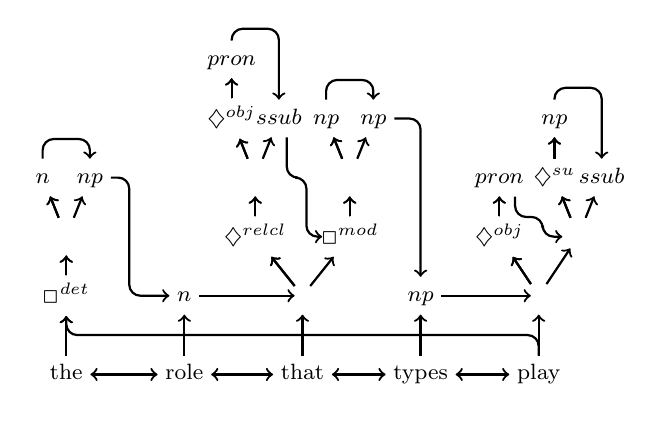
\begin{tikzpicture}
        [tree/.style={dashed},
         ctx/.style={thick, ->, rounded corners},
         ctxbi/.style={thick, <->}]
        \tikzset{every node/.style={outer sep=0pt}}
        	\smaller
        		\node			(w1)				at (-8.5, 0)  		{\hnorm the};
        		\node			(t1_det)			at (-8.5, 1)		{\hnorm $\Box^{det}$};
        		\node			(t1_li)				at (-8.5, 1.75)		{\hnorm $\li$};
        		\node			(t1_n)				at (-8.8, 2.5)		{\hnorm $n$};
        		\node			(t1_np)				at (-8.2, 2.5)		{\hnorm $np$};
        		\node			(w2)				at (-7,0)			{\hnorm role};
        		\node			(t2_n)				at (-7, 1)			{\hnorm $n$};
        		\node			(w3)				at (-5.5, 0)		{\hnorm that};
        		\node			(t3_li1)			at (-5.5, 1)		{\hnorm $\li$};
        		\node			(t3_rc)				at (-6.1, 1.75)		{\hnorm $\diamondsuit^{relcl}$};
        		\node			(t3_mod)			at (-4.9, 1.75)		{\hnorm $\Box^{mod}$};
        		\node			(t3_li2)			at (-6.1, 2.5)		{\hnorm $\li$};
        		\node			(t3_li3)			at (-4.9, 2.5)		{\hnorm $\li$};
        		\node			(t3_obj)			at (-6.4, 3.25)		{\hnorm $\diamondsuit^{obj}$};
        		\node			(t3_pron)			at (-6.4, 4)		{\hnorm $pron$};
        		\node			(t3_ss)				at (-5.8, 3.25)		{\hnorm $ssub$};
        		\node			(t3_np1)			at (-5.2, 3.25)		{\hnorm $np$};
        		\node			(t3_np2)			at (-4.6, 3.25)		{\hnorm $np$};
        		\node			(w4)				at (-4, 0)			{\hnorm types};
        		\node			(t4_np)				at (-4, 1)			{\hnorm $np$};
        		\node			(w5)				at (-2.5, 0)		{\hnorm play};
        		\node			(t5_li1)			at (-2.5, 1)		{\hnorm $\li$};
        		\node			(t5_obj)			at (-3, 1.75)		{\hnorm $\diamondsuit^{obj}$};
        		\node			(t5_pron)			at (-3, 2.5)		{\hnorm $pron$};
        		\node			(t5_li2)			at (-2, 1.75)		{\hnorm $\li$};
        		\node			(t5_su)				at (-2.3, 2.5)		{\hnorm $\diamondsuit^{su}$	};
        		\node			(t5_np)				at (-2.3, 3.25)		{\hnorm $np$};
        		\node			(t5_ss)				at (-1.7, 2.5)		{\hnorm $ssub$};
				%%%% Tree Structure
				\draw[tree]		(t1_det) -- (t1_li) -- (t1_n);
				\draw[tree] 	(t1_li)	-- (t1_np);
				\draw[tree]		(t3_li1) -- (t3_rc) -- (t3_li2) -- (t3_obj) -- (t3_pron);
				\draw[tree] 	(t3_li2) -- (t3_ss);
				\draw[tree]		(t3_li1) -- (t3_mod) -- (t3_li3) -- (t3_np1);
				\draw[tree]		(t3_li3) -- (t3_np2);
				\draw[tree]		(t5_li1) -- (t5_obj) -- (t5_pron);
				\draw[tree]		(t5_li1) -- (t5_li2) -- (t5_su) -- (t5_np);
				\draw[tree]		(t5_li2) -- (t5_ss);
        		%
        		\visible<2->{
        			\draw[ctxbi] (w1) -- (w2);
        			\draw[ctxbi] (w2) -- (w3);
        			\draw[ctxbi] (w3) -- (w4);
        			\draw[ctxbi] (w4) -- (w5);
        		}
        		\visible<3-8>{
        			\draw[ctx] ($(w5.north)$) |- (-4, 0.5) -| ($(t1_det.south)$);
        			\visible<4->{
					\draw[ctx] (t1_det) -- (t1_li);
					}
					\visible<5->{
					\draw[ctx] (t1_li) -- (t1_n);
					}
					\visible<6->{
					\draw[ctx] ($(t1_n.north)$) -- ($(t1_n.north) + (0, 0.25)$) -| ($(t1_np.north)$);
					}
					\visible<7->{
					\draw[ctx] ($(t1_np.east)$) -- ($(t1_np) + (0.5, 0)$) |- ($(t2_n.west)$);
					}
					\visible<8->{
					\draw[ctx] (t2_n) -- (t3_li1);
					\draw[ctx] (t3_li1) -- (t3_rc);
					\draw[ctx] (t3_rc) -- (t3_li2);
					\draw[ctx] (t3_li2) -- (t3_obj);
					\draw[ctx] (t3_obj) -- (t3_pron);
					\draw[ctx] ($(t3_pron.north)$) -- ($(t3_pron.north) + (0, 0.15)$) -| ($(t3_ss.north)$);
					\draw[ctx] ($(t3_ss.south) + (0.1, 0)$) |- ($(-5.45, 2.5)$) -- ($(-5.45, 1.75)$) -- ($(-5.25, 1.75)$);
					\draw[ctx] (t3_mod) -- (t3_li3);
					\draw[ctx] (t3_li3) -- (t3_np1);
					\draw[ctx] ($(t3_np1.north)$) -- ($(t3_np1.north) + (0, 0.25)$) -| ($(t3_np2.north)$);
					\draw[ctx] ($(t3_np2.east)$) -| ($(t4_np.north)$);
					\draw[ctx] (t4_np) -- (t5_li1);
					\draw[ctx] (t5_li1) -- (t5_obj);
					\draw[ctx] (t5_obj) -- (t5_pron);
					\draw[ctx] ($(t5_pron.south) + (0.2, 0)$) |- ($(-2.45, 2)$) -- ($(-2.45, 1.75)$) -- ($(-2.2, 1.75)$);
					\draw[ctx] (t5_li2) -- (t5_su);
					\draw[ctx] (t5_su) -- (t5_np);
					\draw[ctx] ($(t5_np.north)$) -- ($(t5_np.north) + (0, 0.15)$) -| ($(t5_ss.north)$);
        			}
        		}
        		\visible<10->{
        			\draw[ctx] (w1) -- (t1_det);
        			\draw[ctx] (w2) -- (t2_n);
        			\draw[ctx] (w3) -- (t3_li1);
        			\draw[ctx] (w4) -- (t4_np);
        			\draw[ctx] (w5) -- (t5_li1);
					\visible<11->{
						\draw[ctx] (t1_det) -- (t1_li);
						\draw[ctx] (t3_li1) -- (t3_rc);
						\draw[ctx] (t3_li1) -- (t3_mod);
						\draw[ctx] (t5_li1) -- (t5_obj);
						\draw[ctx] (t5_li1) -- (t5_li2);
						\visible<12->{
							\draw[ctx] (t1_li) -- (t1_n);
							\draw[ctx] (t1_li) -- (t1_np);
							\draw[ctx] (t3_rc) -- (t3_li2);
							\draw[ctx] (t3_mod) -- (t3_li3);
							\draw[ctx] (t5_obj) -- (t5_pron);
							\draw[ctx] (t5_li2) -- (t5_su);
							\draw[ctx] (t5_li2) -- (t5_ss);
							\draw[ctx] (t3_li2) -- (t3_obj);
							\draw[ctx] (t3_li2) -- (t3_ss);
							\draw[ctx] (t3_li3) -- (t3_np1);
							\draw[ctx] (t3_li3) -- (t3_np2);
							\draw[ctx] (t5_su) -- (t5_np);
							\draw[ctx] (t3_obj) -- (t3_pron);
						}
					}
				}
        \end{tikzpicture}
\end{frame}


\begin{frame}{Post-modernity}
    \smaller
    neither sequence nor tree but \alert{sequence of trees}
    
    $
    p(\sigma_1, \dots \sigma_m ~ | ~ w_1, \dots w_n) \approx \prod_i^m (\sigma_i~|~\sigma_j : \mathrm{depth}(\sigma_j) < \mathrm{depth}(\sigma_i), w_1,\dots w_n)$\\
    \vfill
    
    	     \centering
        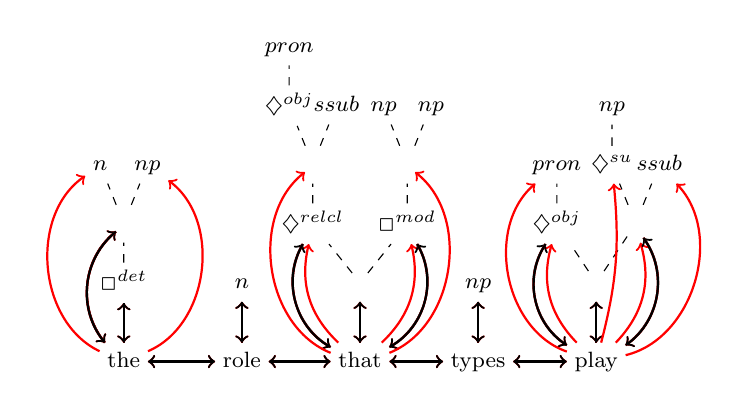
\begin{tikzpicture}
        [state/.style={},
        tree/.style={dashed},
        ctx/.style={thick, ->, rounded corners},
        rctx/.style={thick, <-, rounded corners},
        actx/.style={ctx, red},
        arctx/.style={rctx, red},
        ctxbi/.style={thick, <->},
        actxbi/.style={ctxbi,red}]
        \tikzset{every node/.style={outer sep=0pt}}
        	\smaller
        		\node			(w1)				at (-8.5, 0)  		{\hnorm the};
        		\node			(t1_det)			at (-8.5, 1)		{\hnorm $\Box^{det}$};
        		\node			(t1_li)				at (-8.5, 1.75)		{\hnorm $\li$};
        		\node			(t1_n)				at (-8.8, 2.5)		{\hnorm $n$};
        		\node			(t1_np)				at (-8.2, 2.5)		{\hnorm $np$};
        		\node			(w2)				at (-7,0)			{\hnorm role};
        		\node			(t2_n)				at (-7, 1)			{\hnorm $n$};
        		\node			(w3)				at (-5.5, 0)		{\hnorm that};
        		\node			(t3_li1)			at (-5.5, 1)		{\hnorm $\li$};
        		\node			(t3_rc)				at (-6.1, 1.75)		{\hnorm $\diamondsuit^{relcl}$};
        		\node			(t3_mod)			at (-4.9, 1.75)		{\hnorm $\Box^{mod}$};
        		\node			(t3_li2)			at (-6.1, 2.5)		{\hnorm $\li$};
        		\node			(t3_li3)			at (-4.9, 2.5)		{\hnorm $\li$};
        		\node			(t3_obj)			at (-6.4, 3.25)		{\hnorm $\diamondsuit^{obj}$};
        		\node			(t3_pron)			at (-6.4, 4)		{\hnorm $pron$};
        		\node			(t3_ss)				at (-5.8, 3.25)		{\hnorm $ssub$};
        		\node			(t3_np1)			at (-5.2, 3.25)		{\hnorm $np$};
        		\node			(t3_np2)			at (-4.6, 3.25)		{\hnorm $np$};
        		\node			(w4)				at (-4, 0)			{\hnorm types};
        		\node			(t4_np)				at (-4, 1)			{\hnorm $np$};
        		\node			(w5)				at (-2.5, 0)		{\hnorm play};
        		\node			(t5_li1)			at (-2.5, 1)		{\hnorm $\li$};
        		\node			(t5_obj)			at (-3, 1.75)		{\hnorm $\diamondsuit^{obj}$};
        		\node			(t5_pron)			at (-3, 2.5)		{\hnorm $pron$};
        		\node			(t5_li2)			at (-2, 1.75)		{\hnorm $\li$};
        		\node			(t5_su)				at (-2.3, 2.5)		{\hnorm $\diamondsuit^{su}$	};
        		\node			(t5_np)				at (-2.3, 3.25)		{\hnorm $np$};
        		\node			(t5_ss)				at (-1.7, 2.5)		{\hnorm $ssub$};
				%%%% Tree Structure
				\draw[tree]		(t1_det) -- (t1_li) -- (t1_n);
				\draw[tree] 	(t1_li)	-- (t1_np);
				\draw[tree]		(t3_li1) -- (t3_rc) -- (t3_li2) -- (t3_obj) -- (t3_pron);
				\draw[tree] 	(t3_li2) -- (t3_ss);
				\draw[tree]		(t3_li1) -- (t3_mod) -- (t3_li3) -- (t3_np1);
				\draw[tree]		(t3_li3) -- (t3_np2);
				\draw[tree]		(t5_li1) -- (t5_obj) -- (t5_pron);
				\draw[tree]		(t5_li1) -- (t5_li2) -- (t5_su) -- (t5_np);
				\draw[tree]		(t5_li2) -- (t5_ss);
        		%
        		\alt<4,7>{
      				\draw[actxbi] (w1) -- (w2);
	      			\draw[actxbi] (w2) -- (w3);
    				\draw[actxbi] (w3) -- (w4);
    				\draw[actxbi] (w4) -- (w5);
       			}
      			{   
       				\draw[ctxbi] (w1) -- (w2);
	       			\draw[ctxbi] (w2) -- (w3);
  					\draw[ctxbi] (w3) -- (w4);
   					\draw[ctxbi] (w4) -- (w5);
       			}
        		\visible<2->{
        			\alt<2>{
		        		\draw[actx] (w1) -- (t1_det);
	    	    		\draw[actx] (w2) -- (t2_n);
	        			\draw[actx] (w3) -- (t3_li1);
	        			\draw[actx] (w4) -- (t4_np);
	        			\draw[actx] (w5) -- (t5_li1);
        			}
        			{\invisible<3>{
		        		\draw[ctx] (w1) -- (t1_det);
	    	    		\draw[ctx] (w2) -- (t2_n);
	        			\draw[ctx] (w3) -- (t3_li1);
	        			\draw[ctx] (w4) -- (t4_np);
	        			\draw[ctx] (w5) -- (t5_li1);
        			}}
        		}
        		\visible<3->{
        			\alt<3>{
		        		\draw[arctx] (w1) -- (t1_det);
	    	    		\draw[arctx] (w2) -- (t2_n);
	        			\draw[arctx] (w3) -- (t3_li1);
	        			\draw[arctx] (w4) -- (t4_np);
	        			\draw[arctx] (w5) -- (t5_li1);
        			}
        			{
		        		\draw[rctx] (w1) -- (t1_det);
	    	    		\draw[rctx] (w2) -- (t2_n);
	        			\draw[rctx] (w3) -- (t3_li1);
	        			\draw[rctx] (w4) -- (t4_np);
	        			\draw[rctx] (w5) -- (t5_li1);
        			}
        		}
        		\visible<5->{
        			\alt<5>{
        				\draw[actx] (w1) to[bend left=45] (t1_li);
        				\draw[actx] (w3) to[bend left=30] (t3_rc);
        				\draw[actx] (w3) to[bend right=30] (t3_mod);
						\draw[actx] (w5) to[bend left=30] (t5_obj);
						\draw[actx] (w5) to[bend right=30] (t5_li2);
        			}
        			{\invisible<6>{
    	   				\draw[ctx] (w1) to[bend left=45] (t1_li);
        				\draw[ctx] (w3) to[bend left=45] (t3_rc);
        				\draw[ctx] (w3) to[bend right=45] (t3_mod);
						\draw[ctx] (w5) to[bend left=45] (t5_obj);
						\draw[ctx] (w5) to[bend right=45] (t5_li2);
        			}}
        		}
				\visible<6->{
        			\alt<6>{
        				\draw[arctx] (w1) to[bend left=45] (t1_li);
        				\draw[arctx] (w3) to[bend left=45] (t3_rc);
        				\draw[arctx] (w3) to[bend right=45] (t3_mod);
						\draw[arctx] (w5) to[bend left=45] (t5_obj);
						\draw[arctx] (w5) to[bend right=45] (t5_li2);
        			}
        			{
    	   				\draw[rctx] (w1) to[bend left=45] (t1_li);
        				\draw[rctx] (w3) to[bend left=45] (t3_rc);
        				\draw[rctx] (w3) to[bend right=45] (t3_mod);
						\draw[rctx] (w5) to[bend left=45] (t5_obj);
						\draw[rctx] (w5) to[bend right=45] (t5_li2);
        			}
        		}
        		\visible<8->{
        				\draw[actx] (w1) to[bend left=60] (t1_n);
        				\draw[actx] (w1) to[bend right=60] (t1_np);
        				\draw[actx] (w3) to[bend left=60] (t3_li2);
        				\draw[actx] (w3) to[bend right=60] (t3_li3);
        				\draw[actx] (w5) to[bend left=60] (t5_pron);
        				\draw[actx] (w5) to[bend right=10] (t5_su);
        				\draw[actx] (w5) to[bend right=60] (t5_ss);
        		}
%        		\visible<9->{
%        			\alt<9>{
%        				\draw[arctx] (w1) to[bend left=60] (t1_n);
%        				\draw[arctx] (w1) to[bend right=60] (t1_np);
%        				\draw[arctx] (w3) to[bend left=60] (t3_li2);
%        				\draw[arctx] (w3) to[bend right=60] (t3_li3);
%        				\draw[arctx] (w5) to[bend left=60] (t5_pron);
%        				\draw[arctx] (w5) to[bend right=10] (t5_su);
%        				\draw[arctx] (w5) to[bend right=60] (t5_ss);
%        			}
%        			{
%        				\draw[rctx] (w1) to[bend left=60] (t1_n);
%        				\draw[rctx] (w1) to[bend right=60] (t1_np);
%        				\draw[rctx] (w3) to[bend left=60] (t3_li2);
%        				\draw[rctx] (w3) to[bend right=60] (t3_li3);
%        				\draw[rctx] (w5) to[bend left=60] (t5_pron);
%        				\draw[rctx] (w5) to[bend right=10] (t5_su);
%        				\draw[rctx] (w5) to[bend right=60] (t5_ss);
%        			}
%        		}
        \end{tikzpicture}
        \vfill

		\flushleft
		\textit{(%
			\alt<2->{%
				\alt<2,5,8>{predict}%
				{\alt<3,6>{feedback}{contextualize}}%
			}{encode}%
		)}
\end{frame}

\begin{frame}{DL Jargon}
	\smaller
    \begin{itemize}
        \item \textit{contextualize: states $\to$ states}\\
        \quad \alert{universal transformer encoder w/ relative distance weights}\\
        \quad (many-to-many, update states with neighborhood context)
        \item \textit{predict: state $\to$ nodes}\\
        \quad \alert{token classification w/ unary tree node embeddings}\\
        \quad (one-to-many, predict fringe nodes from current state)
        \item \textit{feedback: nodes $\to$ state}\\
        \quad \alert{heterogeneous dynamic graph attention}\\
        \quad (many-to-one, update state with last predicted nodes)
	\end{itemize} 
\end{frame}

\begin{frame}{Color coded summary}
	\smaller[2]
	{
    \centering
    \begin{tabularx}{1.05\textwidth}{@{}l@{~~~}c@{~~~}c@{~~~}c@{~~~}c@{}}
    \textit{decoder}					& seq2seq[$t$] 				& seq2seq[$\sigma$]				& 	tree					& dynamic graph\\
    \toprule
    \textit{codomain}					& \dr{fixed}				& \dy{open}						& \dg{constrained}			& \dg{constrained}\\
    \textit{context}					& \dg{left}					& \dg{preorder	(global)}		& \dr{ancestors (local)}	& \dg{levels (global)}\\
    \textit{complexity}					& \dy{\# words}				& \dr{\# symbols} 				& \dg{tree depth}			& \dg{tree depth}\\
    \textit{treeness}					& \dr{ignored}				& \dy{implicit}					& \dg{explicit}				& \dg{explicit}\\
    \textit{sequencess}					& \dg{explicit}				& \dy{misaligned}				& \dr{ignored}				& \dg{explicit}\\
    \textit{search?}					& \dg{\cmark}				& \dg{\cmark}					& \dr{\xmark}				& \dy{\textbf{?}}
    \end{tabularx}
    }
    \vfill
    
	\textbf{legend}
	\begin{itemize}
	\item	\dg{green} = good
	\item	\dy{yellow} = meh
	\item	\dr{red} = bad
	\end{itemize}
\end{frame}

%\begin{frame}{Fancy DL Jargon}
%    \smaller 
%    \begin{itemize}
%        \item \textit{contextualize: states $\to$ states}\\
%        \quad \alert{universal transformer encoder w/ relative weights}\\
%        \quad (many-to-many, update states with neighborhood context)
%        \item \textit{predict: state $\to$ nodes}\\
%        \quad \alert{token classification w/ dynamic tree embeddings}\\
%        \quad (one-to-many, predict fringe nodes from current state)
%        \item \textit{feedback: nodes $\to$ state}\\
%        \quad \alert{heterogeneous graph attention}\\
%        \quad (many-to-one, update state with last predicted nodes)
%    \end{itemize} 
%    \vfill
%    \flushright
%    [\href{https://arxiv.org/abs/2203.12235}{Kogkalidis \& Moortgat, ???}]
%\end{frame}

\begin{frame}{Table with numbers}
        \vspace{-10pt}
        \smaller[2]
        \centering
        \begin{tabularx}{0.99\textwidth}{@{}l@{~}L@{}c@{\quad}c@{\quad}c@{\quad}c@{\quad}c@{}}
        & & \multicolumn{5}{c}{\textbf{accuracy} {(\%)}} \\
        \cmidrule(lr){3-7}
        & \multicolumn{1}{c}{\textbf{model}} & {overall} & {frequent} & {uncommon} & {~~rare~~} & {unseen}\\
        \toprule
        \multicolumn{7}{c}{\textit{\textbf{\AE thel} (van Benthem calculus \& dependency modalities, nl)}}\\
        \rowcolor{gray!20}
        & Sequential Transformer      & 83.67 & 84.55 & 64.70 & 50.58 & \fbox{24.55}\\
        % & BERT baseline             & 93.52 & \fbox{94.83} & 71.85 & 38.06 & --\\
        % \rowcolor{gray!20}
        & \textit{this work}        & \fbox{93.67} & \fbox{94.72} & \fbox{73.45} & \fbox{53.83} & 15.78\\   
        \addlinespace
        \multicolumn{7}{c}{\textit{\textbf{TLGBank} (Lambek calculus \& control modalities, fr)}}\\
        \rowcolor{gray!20}
        & ELMo LSTM                 & 93.20 & 95.10 & 75.19 & 25.85 & -- \\
        % & BERT baseline             & \fbox{95.93} & \fbox{96.44} & 81.39 & 47.45 & --\\
        % \rowcolor{gray!20}
        & \textit{this work}        & \fbox{95.93} & \fbox{96.40} & \fbox{81.48} & \fbox{55.37} & \fbox{7.26}\\
        \addlinespace
        \multicolumn{7}{c}{\textit{\textbf{CCGbank} (Combinatory Categorial Grammar, en)}} \\
        \rowcolor{gray!20}
        & Sequential RNN            & 95.10 & 95.48 & 65.76 & 26.02 & 0.00\\
        & Tree Recursive            & 96.09 & 96.44 & 68.10 & \fbox{37.40} & 3.03\\
        % & BERT baseline             & 96.22 & 96.58 & 70.29 & 23.17 & -- \\
        \rowcolor{gray!20}
        & Attentive Convolutions    & 96.25 & \fbox{96.64} & 71.04 & --   & -- \\
        & \textit{this work}         & \fbox{96.29} & 96.61 & \fbox{72.06} & 34.45 & \fbox{4.55}\\
        \addlinespace
        \multicolumn{7}{c}{\textit{\textbf{CCGrebank} (ditto, improved version)}}\\
        \rowcolor{gray!20}
        & Sequential RNN            & 94.44 & 94.93 & 66.90 & 27.41 & 1.23\\
        & Tree Recursive            & 94.70 & 95.11 & 68.86 & 36.76 & \fbox{4.94}\\
        % & BERT baseline             & 94.83 & 95.27 & 68.86 & 23.99 & --\\
        \rowcolor{gray!20}
        & \textit{this work}        & \fbox{95.07} & \fbox{95.45} & \fbox{71.40} & \fbox{37.19} & 3.70\\
        \end{tabularx}
\end{frame}


\section{Parsing}


\begin{frame}{Proof Nets 101}
	\smaller[2]
	
	\begin{minipage}[t][30pt]{1\textwidth}
		\alt<5->{\textbf{Proof Net}\\
			$\equiv$ proof, a proof structure you can navigate
			}
		{
			\alt<3->{
			\textbf{Proof Structure}
			A proof frame \& a bijection between $\dg{+}$ and $\dr{-}$ atoms 
			}{
			\textbf{Proof Frame}
			A bi-colored sequence of decomposed formula assignments.
			\begin{itemize}
				\item[\dg{+}] (sub-)formulas we \textit{\dg{have}}
				\item[\dr{-}] (sub-)formulas we \textit{\dr{need}}
			\end{itemize}
			\vspace{-15pt}
			\flushright $\li$~ \textit{preserves} result and \textit{inverts} argument polarity
			}
		}
	\end{minipage}\\
	\begin{minipage}[t]{1\textwidth}	
		\centering
	     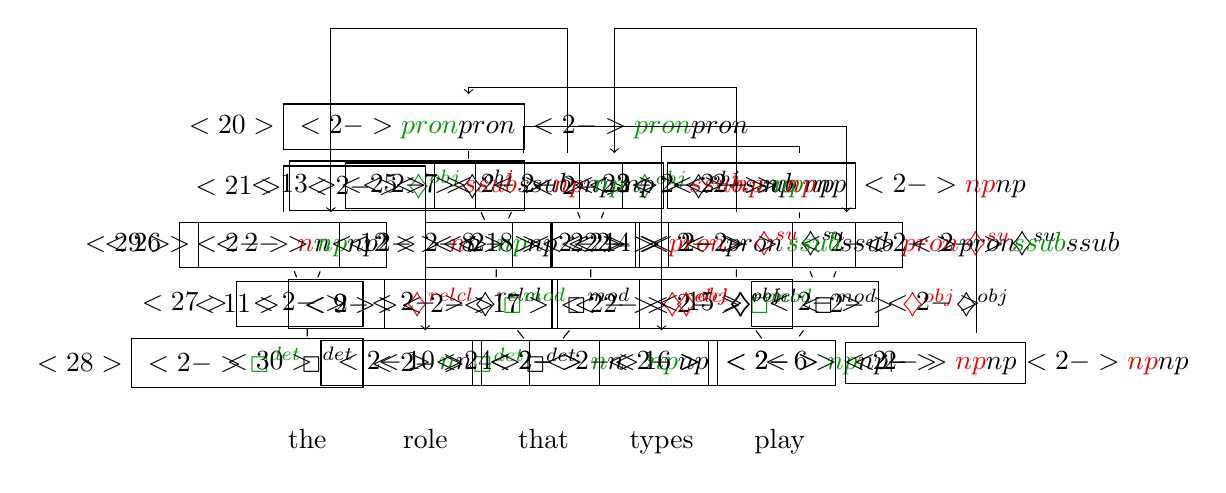
\begin{tikzpicture}
	     [tree/.style={},
	      ctx/.style={thick, ->, rounded corners},
	      ctxbi/.style={thick, <->}]
	      \tikzset{every node/.style={outer sep=0pt}}
	       		\node			(w1)				at (-8.5, 0)  		{\hnorm the};
	       		\node			(t1_det)			at (-8.5, 1)		{$\boxat{28}{\hnorm \dgat{2-}{\Box^{det}}}$};
	       		\node			(t1_li)				at (-8.5, 1.75)		{$\boxat{27}{\hnorm \dgat{2-}{\li}}$};
	       		\node			(t1_n)				at (-8.8, 2.5)		{$\boxat{29}{\hnorm \drat{2-}{n}}$};
	       		\node			(t1_np)				at (-8.2, 2.5)		{$\boxat{26}{\hnorm \dgat{2-}{np}}$};
	       		\node			(w2)				at (-7,0)			{\hnorm role};
	       		\node			(t2_n)				at (-7, 1)			{$\boxat{30}{\hnorm \dgat{2-}{n}}$};
	       		\node			(w3)				at (-5.5, 0)		{\hnorm that};
	       		\node			(t3_li1)			at (-5.5, 1)		{$\boxat{10}{\hnorm \dgat{2-}{\li}}$};
	       		\node			(t3_rc)				at (-6.1, 1.75)		{$\boxat{11}{\hnorm \drat{2-}{\diamondsuit^{relcl}}}$};
	       		\node			(t3_mod)			at (-4.9, 1.75)		{$\boxat{9}{\hnorm \dgat{2-}{\Box^{mod}}}$};
	       		\node			(t3_li2)			at (-6.1, 2.5)		{$\boxat{12}{\hnorm \drat{2-}{\li}}$};
	       		\node			(t3_li3)			at (-4.9, 2.5)		{$\boxat{8}{\hnorm \dgat{2-}{\li}}$};
	       		\node			(t3_obj)			at (-6.45, 3.25)	{$\boxat{21}{\hnorm \dgat{2-}{\diamondsuit^{obj}}}$};
	       		\node			(t3_pron)			at (-6.45, 4)		{$\boxat{20}{\hnorm \dgat{2-}{pron}}$};
	       		\node			(t3_ss)				at (-5.75, 3.25)	{$\boxat{13}{\hnorm \drat{2-}{ssub}}$};
	       		\node			(t3_np1)			at (-5.2, 3.25)		{$\boxat{25}{\hnorm \drat{2-}{np}}$};
	       		\node			(t3_np2)			at (-4.6, 3.25)		{$\boxat{7}{\hnorm \dgat{2-}{np}}$};
	       		\node			(w4)				at (-4, 0)			{\hnorm types};
	       		\node			(t4_np)				at (-4, 1)			{$\boxat{24}{\hnorm \dgat{2-}{np}}$};
	       		\node			(w5)				at (-2.5, 0)		{\hnorm play};
	       		\node			(t5_li1)			at (-2.5, 1)		{$\boxat{16}{\hnorm \dgat{2-}{\li}}$};
	       		\node			(t5_obj)			at (-3.05, 1.75)	{$\boxat{17}{\hnorm \drat{2-}{\diamondsuit^{obj}}}$};
	       		\node			(t5_pron)			at (-3.05, 2.5)		{$\boxat{18}{\hnorm \drat{2-}{pron}}$};
	       		\node			(t5_li2)			at (-1.95, 1.75)	{$\boxat{15}{\hnorm \dgat{2-}{\li}}$};
	       		\node			(t5_su)				at (-2.25, 2.5)		{$\boxat{22}{\hnorm \drat{2-}{\diamondsuit^{su}}}$};
	       		\node			(t5_np)				at (-2.25, 3.25)	{$\boxat{23}{\hnorm \drat{2-}{np}}$};
	       		\node			(t5_ss)				at (-1.65, 2.5)		{$\boxat{14}{\hnorm \dgat{2-}{ssub}}$};
	       		\node			(vdash)				at (-1, 1)			{$\vdash$};
	 	       	\node			(t6_np)				at (0, 1)			{$\boxat{6}{\drat{2-}{np}}$};
				%%%% Tree Structure
				\draw[tree]		(t1_det) -- (t1_li) -- (t1_n);
				\draw[tree] 	(t1_li)	-- (t1_np);
				\draw[tree]		(t3_li1) -- (t3_rc) -- (t3_li2);
				\draw[dashed]	(t3_li2) -- (t3_obj);
				\draw[tree] 	(t3_obj) -- (t3_pron);
				\draw[tree] 	(t3_li2) -- (t3_ss);
				\draw[tree]		(t3_li1) -- (t3_mod) -- (t3_li3) -- (t3_np1);
				\draw[tree]		(t3_li3) -- (t3_np2);
				\draw[tree]		(t5_li1) -- (t5_obj) -- (t5_pron);
				\draw[tree]		(t5_li1) -- (t5_li2) -- (t5_su) -- (t5_np);
				\draw[tree]		(t5_li2) -- (t5_ss);
				%%% Axiom Links
				\visible<4->
				{
				\draw[->] 		(t1_n) -- ($(t1_n) + (0, 1)$) -| (t2_n);	
				\draw[->]		(t3_np1) -- ($(t3_np1) + (0, 2)$) -| (t1_np);
				\draw[->] 		(t5_pron) -- ($(t5_pron) + (0, 2)$) -| (t3_pron);
				\draw[->] 		(t5_np) -- ($(t5_np) + (0, 0.5)$) -| (t4_np);
				\draw[->]		(t3_ss) -- ($(t3_ss) + (0, 0.75)$) -| (t5_ss);
				\draw[<-]    	(t3_np2) -- ($(t3_np2) + (0, 2)$) -| (t6_np);
				}
		\end{tikzpicture}
		
		\smaller
		\alt<32>{
		\flushright
		the bad news: $(\# ~atoms)!$ combinations to consider}{
		\visible<6->{
			\[
			\textcolor{red}{
			\alt<31->{
			\overset{\eta}{\rightsquigarrow}
			\blacktriangledown ^{mod}(\textsf{that}~\vartriangle ^{relcl}\lambda \mathrm{x}.(\textsf{play}~\mathrm{x}~\vartriangle ^{su}\textsf{types}))~
			(\blacktriangledown ^{det}\textsf{the}~\textsf{role})
			}{
			\alt<8->{
				\alt<9->{\blacktriangledown^{mod} (\alt<10->{\textsf{that}~
						\alt<11->{\vartriangle^{relcl}(\alt<12->{\lambda \mathrm{x}.\alt<15->{\alt<16->{\textsf{play}~
						\alt<21->{\vartriangle^{obj}}{}\alt<17->{\triangledown^{obj}\alt<21->{\mathrm{x}}{???}}{???}}{???}~
						\alt<22->{\vartriangle^{su}\alt<24->{\mathsf{types}}{???}}{???}}{???}}{???})}{???}}{???})}{???}
				~\alt<27->{(\alt<28->{\blacktriangledown^{det}\alt<28->{\mathsf{the}}{???}}{???}~\alt<30->{\mathsf{role}}{???})}{???}
			}
			{???}
			}}
			\]
			}
		}
	\end{minipage}%
\end{frame}



\begin{frame}{Proof Nets 102: neural this time}
	\vfill
	
	\smaller
	\alt<3->{
		\alt<8>{
		\noindent 
		\textbf{Sinkhorn-Knopp}\\
		iterative row/column-wise normalization $\rightsquigarrow$ bistochasticity\\
		~\\
		in the log scale:
		\begin{align*}
			& \mathsf{LSE}: \mathbb{R}^{n} \to \mathbb{R} \\
			& \mathsf{LSE}(\mathbf{x})= x^* + log\left(\sum\limits_i \mathsf{exp}(x_i - x^*)\right)	,\quad x^* := \mathsf{max}(\mathbf{x})\\
			\\
			& \mathsf{norm_1}: \mathbb{R}^{n} \to \mathbb{R}^{n}\\
			& \mathsf{norm_1}(\mathbf{x}) = \mathbf{x} - \mathsf{LSE}(\mathbf{x})\\
			\\
			& \mathsf{norm_2}: \mathbb{R}^{n\times n} \to \mathbb{R}^{n\times n}\\
			& \mathsf{norm_2}(X) = \mathsf{norm_1}\left(\mathsf{norm_1}(X)^\top\right)^\top
		\end{align*}
		}
		{
		\centering		
		\larger
		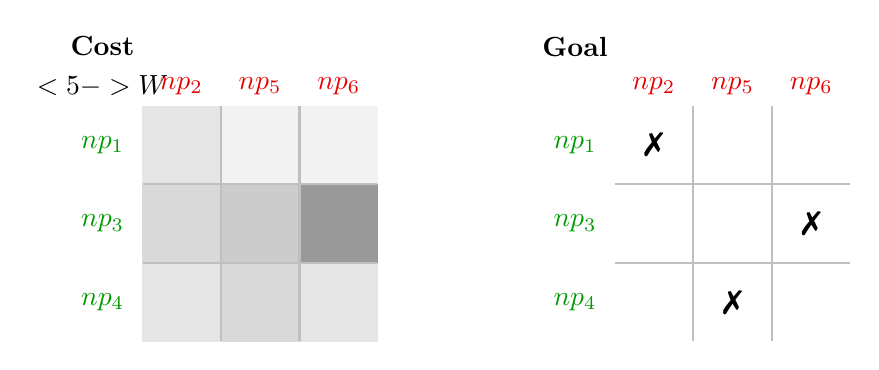
\begin{tikzpicture}
			\visible<4->{
			\node 		(noutput)				at (-3.5, 3.75){\textbf{Cost}};
			\node		(np1)					at (-3.5, 2.5) 	{$\dg{np_1}$};
			\node		(np3)					at (-3.5, 1.5) 	{$\dg{np_3}$};
			\node		(np4)					at (-3.5, 0.5) 	{$\dg{np_4}$};
			\node		(np2)					at (-2.5, 3.25)	{$\dr{np_2}$};
			\node		(np2)					at (-1.5, 3.25)	{$\dr{np_5}$};
			\node		(np2)					at (-0.5, 3.25)	{$\dr{np_6}$};
			\node		(W)						at (-3.5, 3.25)	{$\visible<5->{W}$};
			\alt<8->{
			\fill[gray!80]	(-3, 2) 			rectangle +(1,1);
			\fill[gray!10]	(-3, 1)				rectangle +(1,1);
			\fill[gray!10] 	(-3, 0)				rectangle +(1,1);
			\fill[gray!10] 	(-2, 2)				rectangle +(1,1);
			\fill[gray!20]	(-2, 1)				rectangle +(1,1);
			\fill[gray!70]	(-2, 0)				rectangle +(1,1);
			\fill[gray!10] 	(-1, 2)				rectangle +(1,1);
			\fill[gray!70]	(-1, 1)				rectangle +(1,1);
			\fill[gray!20]	(-1, 0)				rectangle +(1,1);			
			}{
				\visible<5->{
				\fill[gray!20]	(-3, 2) 			rectangle +(1,1);
				\fill[gray!30]	(-3, 1)				rectangle +(1,1);
				\fill[gray!20] 	(-3, 0)				rectangle +(1,1);
				\fill[gray!10] 	(-2, 2)				rectangle +(1,1);
				\fill[gray!40]	(-2, 1)				rectangle +(1,1);
				\fill[gray!30]	(-2, 0)				rectangle +(1,1);
				\fill[gray!10] 	(-1, 2)				rectangle +(1,1);
				\fill[gray!80]	(-1, 1)				rectangle +(1,1);
				\fill[gray!20]	(-1, 0)				rectangle +(1,1);
				}
			}
			\draw[thick, gray!50] (-2.99, 0.01) grid (-0.01,2.99);			
			}
			\node 		(goal)					at (2.5, 3.75)	{\textbf{Goal}};
			\node		(np1)					at (2.5, 2.5) 	{$\dg{np_1}$};
			\node		(np3)					at (2.5, 1.5) 	{$\dg{np_3}$};
			\node		(np4)					at (2.5, 0.5) 	{$\dg{np_4}$};
			\node		(np2)					at (3.5, 3.25)	{$\dr{np_2}$};
			\node		(np2)					at (4.5, 3.25)	{$\dr{np_5}$};
			\node		(np2)					at (5.5, 3.25)	{$\dr{np_6}$};
			\node		(12)					at (3.5, 2.5)	{\larger \xmark};
			\node		(36)					at (5.5, 1.5)	{\larger \xmark};
			\node		(45)					at (4.5, 0.5)	{\larger \xmark};
			\draw[thick, gray!50] (3.01, 0.01) grid (5.99,2.99);			
		\end{tikzpicture}
		}
		\visible<6-7,9->{
		\vfill
		\noindent
		\textbf{LAP}: Find bijection $f: \dg{P} \to \dr{N}$ s.t. $\sum\limits_{p \in P} Cost\left(p, f(p)\right)$ max.\\
		\visible<7->{
		\begin{itemize}
			\item[\alt<9->{\dg{\checkmark}}{\textbf{?}}] boundedness \visible<9->{\textit{ : negative in the log scale}}
			\item[\alt<10->{\dg{\checkmark}}{\textbf{?}}] backprop \visible<10->{\textit{ : NLL /w straight-through estimator}}
		\end{itemize}
		}
		}
	}
	{
		\centering
		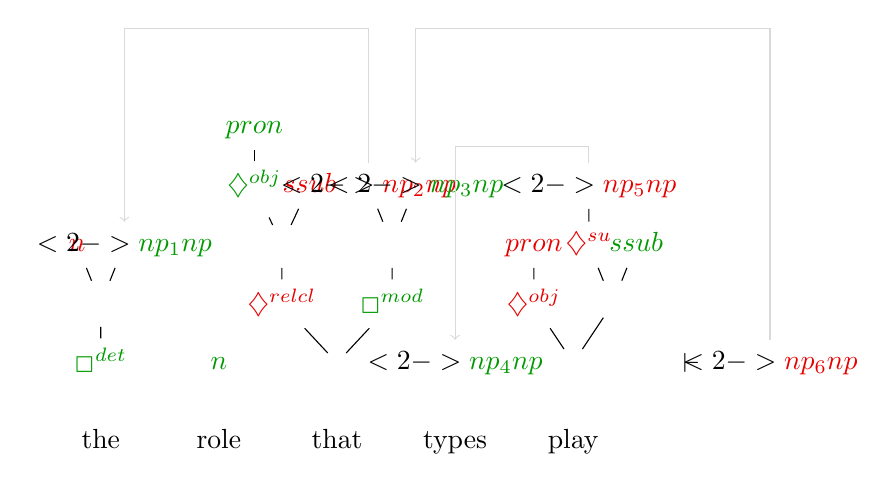
\begin{tikzpicture}
	    [tree/.style={},
	     ctx/.style={thick, ->, rounded corners},
	     ctxbi/.style={thick, <->}]
		\tikzset{every node/.style={outer sep=0pt}}
	    	\node			(w1)				at (-8.5, 0)  		{\hnorm the};
	       	\node			(t1_det)			at (-8.5, 1)		{${\hnorm \dg{\Box^{det}}}$};
	       	\node			(t1_li)				at (-8.5, 1.75)		{${\hnorm \dg{\li}}$};
	       	\node			(t1_n)				at (-8.8, 2.5)		{${\hnorm \dr{n}}$};
	       	\node			(t1_np)				at (-8.2, 2.5)		{$\alt<2->{\hnorm \dg{np_1}}{\hnorm \dg{np}}$};
	       	\node			(w2)				at (-7,0)			{\hnorm role};
	       	\node			(t2_n)				at (-7, 1)			{${\hnorm \dg{n}}$};
	       	\node			(w3)				at (-5.5, 0)		{\hnorm that};
	       	\node			(t3_li1)			at (-5.5, 1)		{${\hnorm \dg{\li}}$};
	       	\node			(t3_rc)				at (-6.2, 1.75)		{${\hnorm \dr{\diamondsuit^{relcl}}}$};
	       	\node			(t3_mod)			at (-4.8, 1.75)		{${\hnorm \dg{\Box^{mod}}}$};
	       	\node			(t3_li2)			at (-6.2, 2.5)		{${\hnorm \dr{\li}}$};
	       	\node			(t3_li3)			at (-4.8, 2.5)		{${\hnorm \dg{\li}}$};
	       	\node			(t3_obj)			at (-6.55, 3.25)	{${\hnorm \dg{\diamondsuit^{obj}}}$};
	       	\node			(t3_pron)			at (-6.55, 4)		{${\hnorm \dg{pron}}$};
	       	\node			(t3_ss)				at (-5.85, 3.25)	{${\hnorm \dr{ssub}}$};
	       	\node			(t3_np1)			at (-5.1, 3.25)		{$\alt<2->{\hnorm \dr{np_2}}{\hnorm \dr{np}}$};
	       	\node			(t3_np2)			at (-4.5, 3.25)		{$\alt<2->{\hnorm \dg{np_3}}{\hnorm \dg{np}}$};
	       	\node			(w4)				at (-4, 0)			{\hnorm types};
	       	\node			(t4_np)				at (-4, 1)			{$\alt<2->{\hnorm \dg{np_4}}{\hnorm \dg{np}}$};
	       	\node			(w5)				at (-2.5, 0)		{\hnorm play};
	       	\node			(t5_li1)			at (-2.5, 1)		{${\hnorm \dg{\li}}$};
	       	\node			(t5_obj)			at (-3, 1.75)		{${\hnorm \dr{\diamondsuit^{obj}}}$};
	       	\node			(t5_pron)			at (-3, 2.5)		{${\hnorm \dr{pron}}$};
	       	\node			(t5_li2)			at (-2, 1.75)		{${\hnorm \dg{\li}}$};
	       	\node			(t5_su)				at (-2.3, 2.5)		{${\hnorm \dr{\diamondsuit^{su}}}$};
	        \node			(t5_np)				at (-2.3, 3.25)		{$\alt<2->{\hnorm \dr{np_5}}{\hnorm \dr{np}}$};
	       	\node			(t5_ss)				at (-1.7, 2.5)		{${\hnorm \dg{ssub}}$};
	   		\node			(vdash)				at (-1, 1)			{$\vdash$};
	 	    \node			(t6_np)				at (0, 1)			{$\alt<2->{\hnorm \dr{np_6}}{\hnorm \dr{np}}$};
			%%%% Tree Structure
			\draw[tree]		(t1_det) -- (t1_li) -- (t1_n);
			\draw[tree] 	(t1_li)	-- (t1_np);
			\draw[tree]		(t3_li1) -- (t3_rc) -- (t3_li2);
			\draw[dashed]	(t3_li2) -- (t3_obj);
			\draw[tree] 	(t3_obj) -- (t3_pron);
			\draw[tree] 	(t3_li2) -- (t3_ss);
			\draw[tree]		(t3_li1) -- (t3_mod) -- (t3_li3) -- (t3_np1);
			\draw[tree]		(t3_li3) -- (t3_np2);
			\draw[tree]		(t5_li1) -- (t5_obj) -- (t5_pron);
			\draw[tree]		(t5_li1) -- (t5_li2) -- (t5_su) -- (t5_np);
			\draw[tree]		(t5_li2) -- (t5_ss);
			%%% Axiom Links
			\draw[->, gray!30]		(t3_np1) -- ($(t3_np1) + (0, 2)$) -| (t1_np);
			\draw[->, gray!30] 		(t5_np) -- ($(t5_np) + (0, 0.5)$) -| (t4_np);
			\draw[<-, gray!30]    	(t3_np2) -- ($(t3_np2) + (0, 2)$) -| (t6_np);
	\end{tikzpicture}
	}	
\end{frame}

\begin{frame}{A note on complexity}
	\vfill

	\noindent
	\smaller
	Forward pass of 64 matrix-batches, 3 Sinkhorn iterations
	
	\centering
	\includegraphics[width=1\textwidth, trim=0 0 0 5pt, clip]{benchmark}
\end{frame}

\begin{frame}[plain]{}
	\centering
	\includegraphics[width=0.375\textwidth]{thinking2.png}
	
	\larger
	\vfill
	constant decoding + constant linking = ???		
\end{frame}

\end{document}
